\documentclass[times, utf8, zavrsni, numeric]{fer}
\usepackage{booktabs}
\usepackage{amsmath}
\usepackage{algorithm}
\usepackage{algorithmic}
% \usepackage{pdfpages}

\begin{document}

% TODO: Navedite broj rada.
\thesisnumber{1160}

% TODO: Navedite naslov rada.
\title{Algoritmi za brzo učenje na neprijateljskim primjerima}

% TODO: Navedite vaše ime i prezime.
\author{Dominik Jambrović}

\maketitle

% Ispis stranice s napomenom o umetanju izvornika rada. Uklonite naredbu \izvornik ako želite izbaciti tu stranicu.
% \izvornik
% 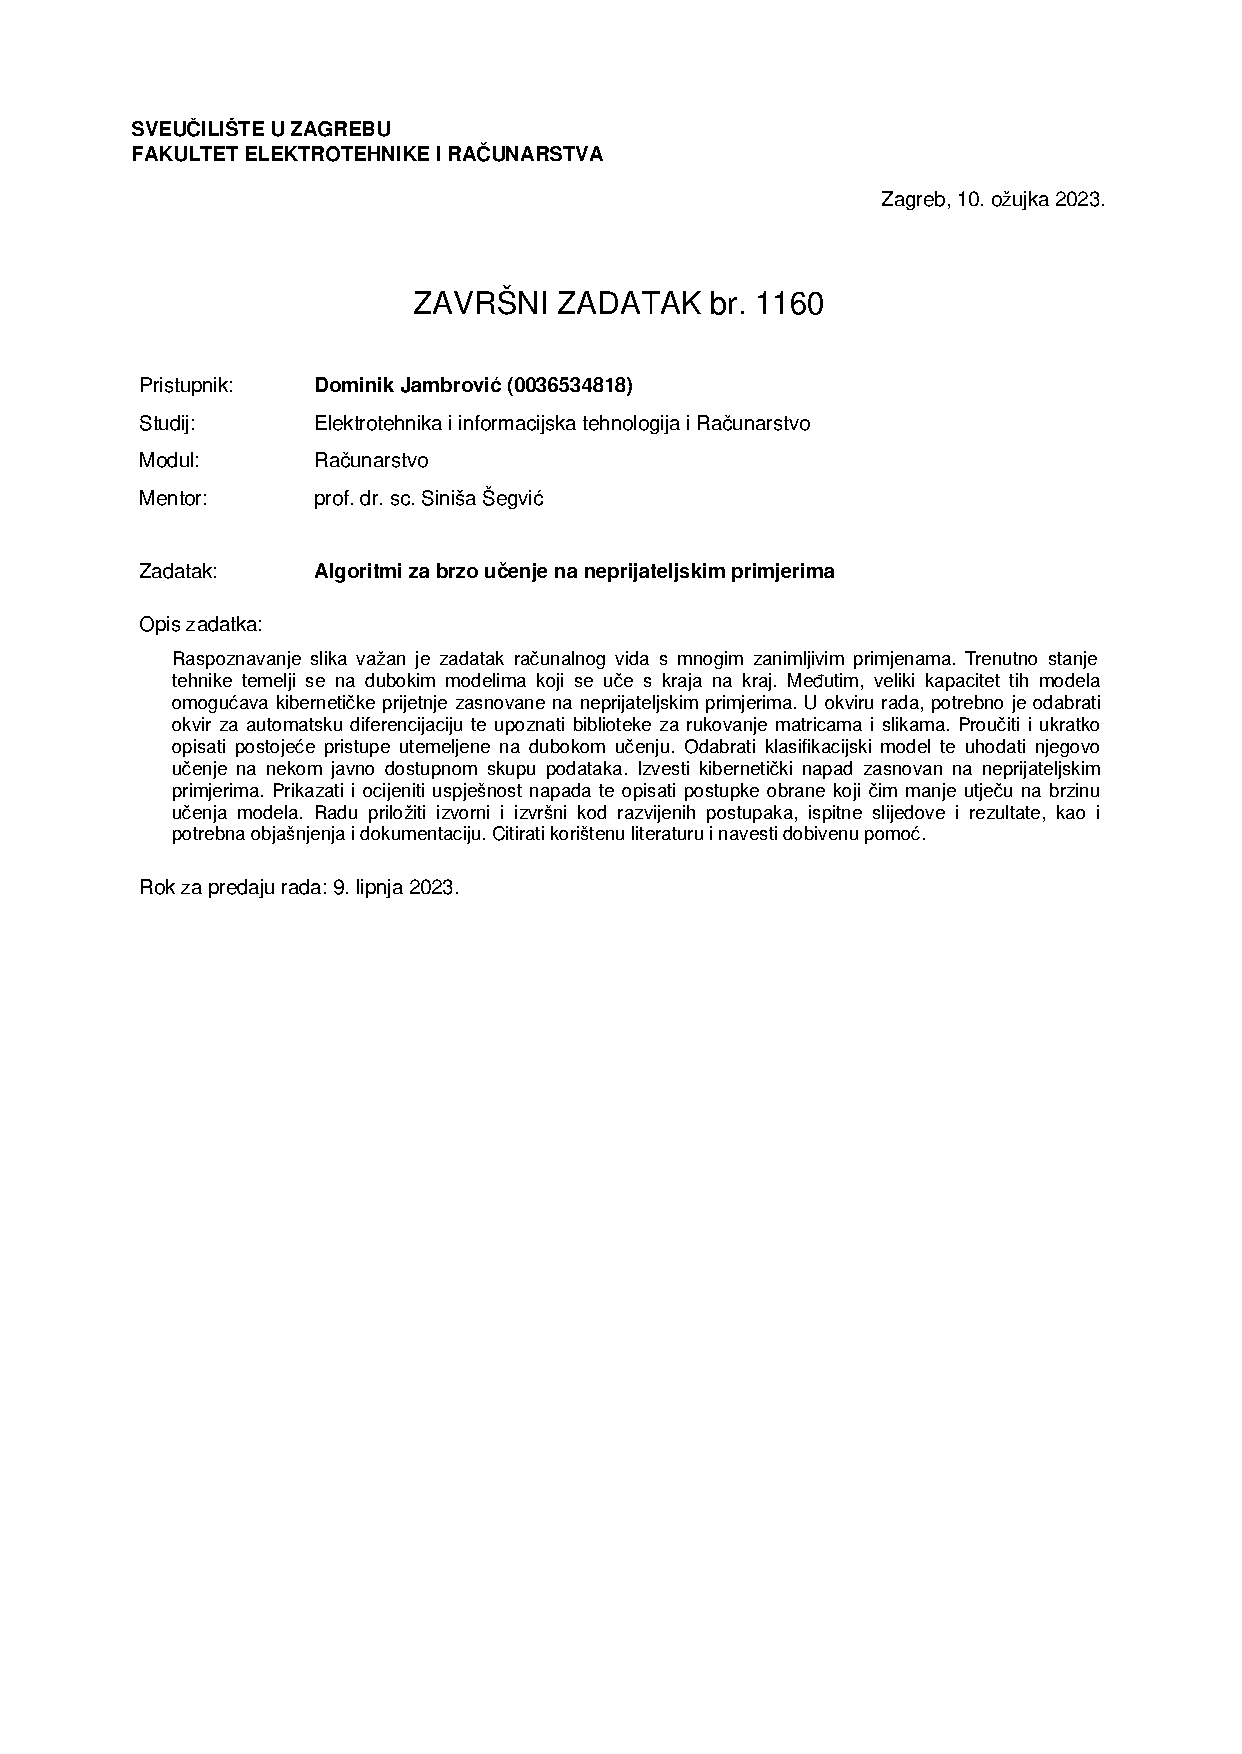
\includepdf[pages={1}]{zadatak.pdf}

\zahvala{Zahvaljujem svojoj obitelji radi podrške tijekom studiranja, kao i prof. dr. sc. Siniši Šegviću te mag. ing. Ivanu Grubišiću na pomoći tijekom izrade završnog rada.}

\tableofcontents

\chapter{Uvod}
Velik broj problema s kojima se danas susrećemo takve su prirode da ne znamo kako ih riješiti koristeći klasičan, algoritamski pristup. Razlog tome često leži u činjenici da ne znamo ni kako mi sami rješavamo te probleme, 
a jedan od najčešćih primjera za to je raspoznavanje tj.\ klasifikacija slika.
Jedno od mogućih rješenja takvih problema je korištenje umjetnih neuronskih mreža - mreža sastavljenih od velikog broja povezanih jedinica (neurona) koje obavljaju veoma jednostavne operacije.

Razvojem dubokih neuronskih mreža došlo je do ubrzanog napretka u području računalnog vida. Računalni vid područje je umjetne inteligencije koje se bavi problemima poput klasifikacije 2D slika. 
Sve većom popularizacijom i korištenjem dubokih modela u sustavima različitih namjena, u pitanje se dovodi sigurnost takvih modela -
ako model želimo koristiti u automobilima s ciljem detekcije pješaka i vozila, model mora moći dobro generalizirati, kao i biti robustan. Takav model ne bi smio mijenjati svoje odluke na temelju veoma malih promjena na ulazu -
na primjeru prometa, želimo da model točno detektira pješaka, bez obzira nosi li on kapu ili ne.

Kako bi ostvarili robusnost modela, predložene su brojne tehnike, a jedna od najpopularnijih je robusno učenje tj.\ učenje na neprijateljskim primjerima. 
Kada su u pitanju modeli koji brzo uče, robusno učenje prihvatljivo je rješenje za postizanje robusnih modela otpornih na napade. 
Ipak, kada su u pitanju veći modeli za koje učenje traje veoma dugo, obično robusno učenje često je neprihvatljivo. 
U tu svrhu, razvijene su metode koje ubrzavaju robusno učenje. U ovome radu, razmatrat ćemo tri takve metode: besplatno robusno učenje~\cite{shafahi2019adversarial}, brzo robusno učenje~\cite{wong2020fast} i
nadogradnju na brzo robusno učenje (FastAdv+ i FastAdvW,~\cite{li2020towards}). 

Uz to, razmatrat ćemo i otpornost naučenih modela na zatrovane podatke. Zatrovani podatci ulazi su izmijenjeni s ciljem navođenja modela na neočekivano ponašanje. 
Uvođenjem takve ranjivosti u model, napadači mogu neprimijećeno postići proizvoljne ciljeve poput izbjegavanja detekcije ili pogrešne klasifikacije.

\chapter{Neuronske mreže}
\section{Općenito o neuronskim mrežama}
Umjetne neuronske mreže veoma su popularan alat za rješavanje kompleksnih problema za koje je teško modelirati ili formalizirati znanje. 
Predstavnik su konektivističkog pristupa umjetnoj inteligenciji~\cite{uui2020} koji se zasniva na oblikovanju sustava inspiriranih građom mozga.

Problemi koje rješavamo umjetnim neuronskim mrežama svrstavaju se u dvije glavne kategorije:
\begin{enumerate}
    \item klasifikacija 
    \item regresija
\end{enumerate}

Kada su u pitanju klasifikacijski problemi, cilj nam je svrstati ulaz u jedan od mogućih razreda. 
Pritom je na izlazu često korišteno jednojedinično kodiranje - ako ulaze svrstavamo u 10 razreda, u izlaznom sloju mreže bit će 10 neurona, a aktivacija jednog od njih predstavljat će rezultat klasifikacije.

S druge strane, kod regresijskih problema cilj nam je što bolje aproksimirati neku, modelu nepoznatu, funkciju. Za ovakve probleme, često nam je dovoljan jedan neuron u izlaznom sloju. 
Taj neuron na izlazu bi trebao davati predviđenu vrijednost funkcije za neki, do sada neviđeni, ulaz.

Da bi neuronska mreža mogla rješavati takve probleme, važno nam je da može učiti na temelju predočenih podataka. Učenje neuronske mreže odvija se izmjenom težina pojedinih neurona (time znanje implicitno ugrađujemo u našu mrežu).
Kako bismo detaljnije mogli govoriti o učenju i arhitekturama neuronskih mreža, važno je ukratko opisati neuron - osnovnu gradivnu jedinicu svake mreže.
\pagebreak
\section{Umjetni neuron}
Umjetni neuroni predstavljaju jednostavne procesne jedinice koje modeliraju ponašanje prirodnih neurona. Osnovni neuron akumulira vrijednosti na ulazu pomnožene težinama, 
akumuliranoj vrijednosti dodaje pomak te na kraju istu propušta kroz prijenosnu (aktivacijsku) funkciju. Ponašanje jednog neurona možemo modelirati jednadžbom:

\begin{equation}
    o = f(\sum_{i=1}^{n}x_{i} \cdot w_{i} + b)
    \label{eq:neuron}
\end{equation}
\\
\noindent pri čemu $x$ označava pojedine ulaze, $w$ težine na pripadnim ulazima, $b$ pomak te $f$ prijenosnu funkciju. 

\section{Prijenosne funkcije}
Neki od najranijih modela umjetnog neurona kao prijenosnu funkciju koristili su funkciju identiteta (ADELINE-neuron) te funkciju skoka (TLU-perceptron).
S vremenom su korištene i razvijene brojne druge prijenosne funkcije poput sigmoidalne funkcije definirane kao:

\begin{equation}
    sigmoid(x) = \frac{1}{1 + e^{-x}}
    \label{eq:sigmoid}
\end{equation}
\\
Sigmoidalna funkcija značajna je zbog svojstva derivabilnosti nad cijelom svojom domenom. Ovo svojstvo važno je za brojne optimizacijske postupke.
Uz nju, danas je veoma značajna i zglobnica (ReLU - engl.\ \textit{Rectified Linear Unit}) koju možemo prikazati na sljedeći način:

\begin{equation}
    relu(x) = max(0, x)
    \label{eq:relu}
\end{equation}
\\
Osim navedenih prijenosnih funkcija, korištena je i softmax funkcija koju jednadžbom možemo prikazati kao:

\begin{equation}
    softmax(x_{i}) = \frac{e^{x_{i}}}{\sum_{j=1}^{n}e^{x_{j}}}
    \label{eq:softmax}
\end{equation}
\\
\pagebreak

Softmax funkcija poopćenje je sigmoidalne funkcije, a često se koristi kao zadnja prijenosna funkcija u neuronskim mrežama korištenim za klasifikaciju.
Korištenjem te funkcije u zadnjem sloju, na izlazu mreže imat ćemo vjerojatnosti klasifikacije u pojedini od razreda. Ovo svojstvo korisno nam je kada kao funkciju gubitka koristimo unakrsnu entropiju.

Važno je primijetiti da ako je prijenosna funkcija linearna, cijeli neuron može postići isključivo linearnu transformaciju. 
Kako bi umjetnim neuronima mogli modelirati kompleksnije funkcije, koristimo nelinearne prijenosne funkcije poput sigmoidalne funkcije i zglobnice. 
Pritom je za duboke neuronske mreže s velikim brojem slojeva često korištena upravo zglobnica - 
sigmoidalna funkcija za takve mreže nije prikladna zbog problema nestajućeg gradijenta (engl.\ \textit{vanishing gradient problem}) koji nastaje tijekom učenja temeljenog na gradijentnim metodama.

\section{Arhitektura umjetne neuronske mreže}
Kada je za neki problem potrebno koristiti više od jednog osnovnog neurona, neurone povezujemo u mrežu. Pritom kažemo da se neuronska mreža sastoji od nekolicine slojeva:
\begin{enumerate}
    \item ulazni sloj
    \item skriveni slojevi
    \item izlazni sloj
\end{enumerate}
Iako ulazni sloj predstavljamo neuronima, oni, za razliku od neurona u skrivenim slojevima i izlaznom sloju, ne obavljaju nikakve transformacije - možemo reći da predstavljaju ulazni podatak.
Veličina ulaznog sloja govori nam o dimenzijama ulaznih podataka, a veličina izlaznog sloja u slučaju problema klasifikacije često nam govori o broju razreda u koje klasificiramo ulaz. 

\pagebreak
\begin{figure}[htb]
    \centering
    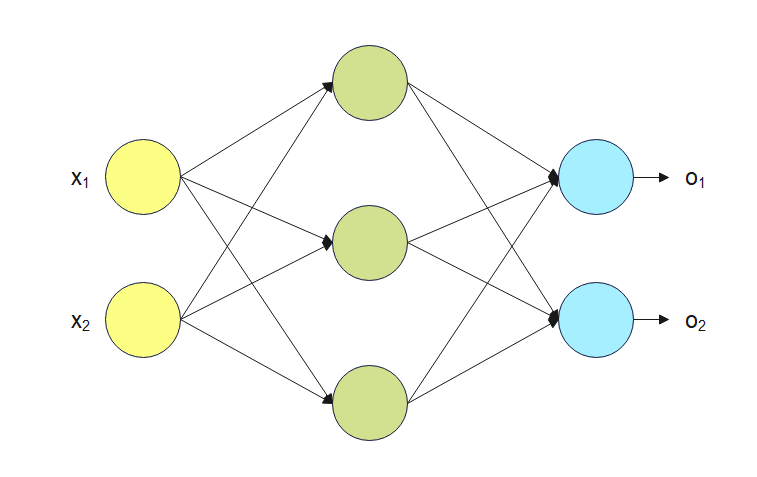
\includegraphics{basic_nn_labeled.png}
    \caption{2x3x2 arhitektura umjetne neuronske mreže}
    \label{fig:basic_nn}
\end{figure}

Na slici~\ref{fig:basic_nn} moguće je vidjeti primjer arhitekture umjetne neuronske mreže. 
Neuroni označeni žutom bojom predstavljaju ulazni sloj, neuroni označeni zelenom bojom skriveni sloj, a neuroni označeni plavom bojom izlazni sloj. 
Ovakvu arhitekturu mreže skraćeno možemo označiti kao 2x3x2 neuronsku mrežu. Pritom brojke označavaju broj neurona u pojedinom sloju (ulazni sloj je prvi sloj mreže).

Za ovakvu mrežu kažemo da je unaprijedna potpuno-povezana mreža. 
Pojam unaprijedna mreža označava to da ne postoje veze iz dubljih slojeva prema plićim slojevima, a pojam potpuno-povezana mreža označava to da svaki neuron ima vezu sa svakim neuronom iz prethodnog sloja.
Uz to, svi neuroni imaju i dodatnu težinu zvanu pomak (nije prikazano na slici ~\ref{fig:basic_nn}). Djelovanje jednog sloja mreže sažeto možemo prikazati kao:

\begin{equation}
    \pmb{h}_{i} = f(\pmb{W}_{i} \cdot \pmb{h}_{i-1} + \pmb{b}_{i})
    \label{eq:nn_layer}
\end{equation}
\\
pri čemu $W_{i}$ predstavlja težine trenutnog sloja, $b_{i}$ pomake trenutnog sloja, $h_{i-1}$ izlaz iz prethodnog sloja, $f$ prijenosnu funkciju primijenjenu na svaki element te $h_{i}$ izlaz iz trenutnog sloja.
Korištenjem takve formule za svaki sloj mreže, na kraju ćemo dobiti izlaz mreže za neki proizvoljni ulaz. Ovo nazivamo unaprijednim prolazom.

\section{Učenje neuronske mreže}
Kako bismo mogli koristiti proizvoljnu mrežu za probleme klasifikacije ili regresije, potrebno ju je prvo naučiti. 
Kao što je već prethodno rečeno, učenje neuronske mreže odgovara izmjeni težina pojedinih neurona, a najčešće se postiže algoritmom propagacije pogreške unatrag~\cite{Goodfellow-et-al-2016}.
Da bismo mogli znati kako trebamo izmijeniti težine neurona, prvo trebamo znati koliko naš model griješi. Mjera greške naziva se gubitak, a računa se na temelju izlaza modela i očekivanog (točnog) izlaza.
Za izračun gubitka često je korištena unakrsna entropija koju možemo definirati kao:

\begin{equation}
    H(P^{*}|P) = -\sum_{i}P^{*}(i) \cdot \log{P(i)}
    \label{eq:cross_entropy}
\end{equation}
\\
pri čemu $P^{*}(i)$ označava distribuciju očekivanog izlaza, a $P(i)$ distribuciju izlaza modela.
Jednom kada znamo iznos gubitka, koristeći optimizatore poput stohastičkog gradijentnog spusta (SGD) ili Adam optimizatora~\cite{kingma2014adam} možemo poboljšati naš model. 
Pritom nam je za optimizacijski postupak veoma često potreban gradijent funkcije gubitka po parametrima modela, a izračunavamo ga uzastopnom primjenom pravila ulančavanja koje u svojem najjednostavnijem obliku možemo definirati kao:

\begin{equation}
    \frac{dz}{dx} = \frac{dz}{dy} \cdot \frac{dy}{dx}
    \label{eq:chain_rule}
\end{equation}
\\
U slučaju stohastičkog gradijentnog spusta, iterativno ažuriramo težine modela na temelju iznosa gradijenta funkcije gubitka, kao i stope učenja. Sažeto postupak stohastičkog gradijentnog spusta možemo prikazati jednadžbom:

\begin{equation}
    w_{i+1} := w_{i} - \eta \cdot \nabla_{w} \cdot L(w_{i}, x)
    \label{eq:sgd}
\end{equation}
\\
pri čemu $w_{i}$ označava jednu od težina modela u trenutnoj iteraciji, $w_{i+1}$ istu težinu u sljedećoj iteraciji, $L(w_{i}, x)$ funkciju gubitka, a $\eta$ stopu učenja. 
Stopa učenja mali je pozitivni broj pomoću kojeg možemo kontrolirati iznos promjene težina po iteracijama. Iterativnim ponavljanjem ovakvog postupka minimiziramo iznos funkcije gubitka, time dobivajući što bolju mrežu.
Kod stohastičkog gradijentnog spusta, iteracije mogu biti predstavljene pojedinačnim ulazima ili mini-grupama. Zbog činjenice da SGD pohranjuje gradijent za male ulaze, ovaj optimizacijski postupak zahtijeva malo memorije.

Nakon učenja mreže na skupu za učenje, evaluirat ćemo performanse mreže na neviđenom skupu zvanom skup za testiranje (engl.\ \textit{test set}). Često korištena mjera za kvalitetu modela je točnost definirana kao:

\begin{equation}
    accuracy = \frac{correct}{total}
    \label{eq:accuracy}
\end{equation}
\\
pri čemu $correct$ označava broj točno klasificiranih primjera, $total$ ukupan broj primjera, a $accuracy$ točnost.
Uz točnost, postoje i brojne druge mjere kvalitete modela. Neke od njih su preciznost (engl.\ \textit{precision}), odziv (engl.\ \textit{recall}) i matrica zabune (engl.\ \textit{confusion matrix}).

\section{Duboke neuronske mreže}
Ako želimo rješavati složenije probleme koristeći umjetne neuronske mreže sa samo jednim skrivenim slojem, suočit ćemo se s problemom - broj neurona potreban kako bi umjetna neuronska mreža mogla obavljati svoju zadaću bit će prevelik.
Uz to, korištenjem širokog modela s velikim brojem neurona u skrivenom sloju teško ćemo postići svojstvo generalizacije jer će se model lako prenaučiti i zapamtiti ulazne podatke. 

Zbog tih razloga, veoma su popularne duboke neuronske mreže~\cite{Goodfellow-et-al-2016}. Duboke neuronske mreže, za razliku od mreža sa samo jednim skrivenim slojem, imaju nekolicinu skrivenih slojeva. 
Pritom za rješavanje složenijih problema duboke mreže trebaju imati značajno manje neurona po sloju naspram mreže sa samo jednim skrivenim slojem. 
Zasebni slojevi mreže naučit će prepoznavati zasebne značajke ulaza, a njihovom kombinacijom mreža će moći postići uspješnu klasifikaciju.

Ipak, postoje i određene mane dubokih neuronskih mreža. Jedna od mana činjenica je da je za propagaciju pogreške unazad kod ovakvih mreža potrebno množiti gradijente. 
U slučaju da kao prijenosnu funkciju koristimo sigmoidalnu funkciju, ovo lako vodi do problema nestajućeg gradijenata zbog kojega težine neurona u plitkim slojevima nećemo moći ispravno izmijeniti.
Uz problem nestajućeg gradijenta, postoji i problem eksplodirajućeg gradijenta (engl.\ \textit{exploding gradient problem}) koji se pojavljuje kod nekih drugih prijenosnih funkcija od kojih je najpoznatija upravo zglobnica (ReLU).
Još jedna mana dubokih neuronskih mreža činjenica je da kako bismo kvalitetno naučili duboku mrežu moramo imati veoma velik skup podataka.

\section{Konvolucijske mreže}
Za probleme s velikim dimenzijama ulaza, potpuno-povezane mreže imaju izuzetno velik broj parametara tj.\ težina neurona. 
Učenje ovakvih modela zahtijeva veliku količinu memorije, a i općenito je sporo. 
Uz to, potpuno-povezane mreže osjetljive su na translaciju ulaza: ako učimo mrežu da klasificira slike vozila te nakon učenja mreži predočimo translatiranu sliku iz skupa za učenje, mreža tu sliku neće nužno moći ispravno klasificirati jer je za nju to potpuno novi podatak.
Ovo svojstvo proizlazi iz činjenice da je svaki neuron ovisan o svakom neuronu iz prethodnog sloja.

Kako bi doskočili ovim problemima, uvedene su konvolucijske mreže~\cite{o2015introduction}. 
Za razliku od potpuno-povezanih mreža, ovdje aktivacija neurona ne ovisi o svim neuronima iz prethodnog sloja, već samo o malom rasponu neurona iz prethodnog sloja. 
Time konvolucijska mreža ima značajno manje parametara naspram potpuno-povezane mreže iste dubine, a postiže i svojstvo translacijske invarijantnosti.
Ova svojstva konvolucijska mreža postiže zamjenom standardnog množenja matrica operacijom konvolucije s jezgrom (engl.\ \textit{kernel}). 
Općenito govoreći, operaciju konvolucije za dvije funkcije $f, g$ možemo definirati kao:

\begin{equation}
    (f * g)(t) := \int_{-\infty}^{\infty}f(\tau) \cdot g(t-\tau)d\tau
    \label{eq:convolution}
\end{equation}
\\
Operacija konvolucije opisuje nam kako se izgled jedne funkcije mijenja pod utjecajem druge funkcije, 
a definirana je kao integral umnoška funkcija nakon što je jedna reflektirana i translatirana. 
Uz operaciju konvolucije postoji i unakrsna korelacija definirana kao:

\begin{equation}
    (f \star g)(t) := \int_{-\infty}^{\infty}f(\tau) \cdot g(t+\tau)d\tau
    \label{eq:convolution}
\end{equation}
\\
Važno je primijetiti da je glavna razlika između te dvije operacije izostajanje reflektiranja jedne od funkcija u slučaju operacije unakrsne korelacije. 
Kada kod konvolucijskih mreža govorimo o konvoluciji, gotovo uvijek se zapravo misli na unakrsnu korelaciju.

Kako bismo što jednostavnije objasnili konvoluciju, koristit ćemo primjer s 2D konvolucijom.
U tom slučaju, jezgra s kojom se provodi konvolucija mala je kvadratna matrica s težinama koje učenjem izmjenjujemo. Skalarnim produktom dijelova ulazne matrice i jezgre dobivamo izlaz konvolucijskog sloja.
Pritom se jezgra pomiče po ulaznoj matrici, a rezultati skalarnog produkta zapisuju se u novu matricu koju zovemo mapa značajki.

\pagebreak
\begin{figure}[htb]
    \centering
    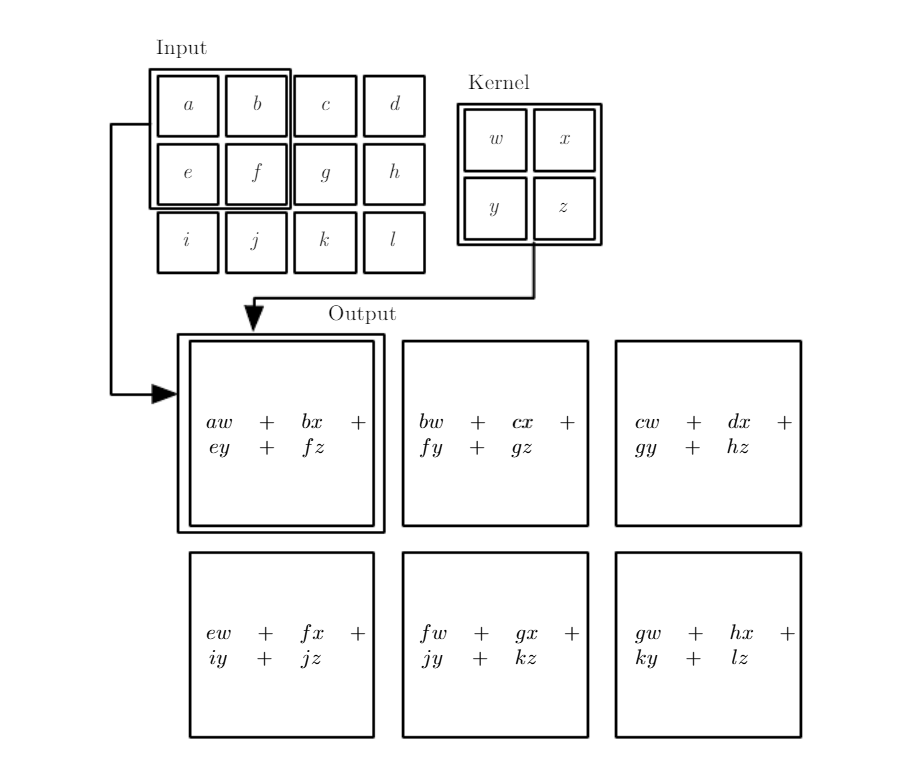
\includegraphics[scale=0.5]{convolution.png}
    \caption{Primjer 2D konvolucije. Preuzeto iz \cite{Goodfellow-et-al-2016}}
    \label{fig:convolution}
\end{figure}

Na slici~\ref{fig:convolution} možemo vidjeti rezultat 2D konvolucije s ulaznom matricom veličine 3x4 i jezgrom dimenzija 2x2. 
Mapa značajki nastala kao rezultat ove konvolucije dimenzija je 2x3. Primijetimo da će izlaz konvolucijskog sloja uvijek biti manjih dimenzija naspram ulaza.
Uz to, vrijednosti na rubovima matrice ulaza manje će doprinijeti rezultatu naspram vrijednosti koje su dalje od rubova.

Kako bismo imali veću kontrolu nad dimenzijama izlaza, kao i utjecajem vrijednosti na rubovima matrice ulaza, često koristimo nadopunjavanje nulama (engl.\ \textit{zero padding}).

\begin{figure}[htb]
    \centering
    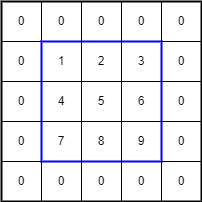
\includegraphics[scale=0.5]{zero_padding.png}
    \caption{Primjer nadopunjavanja 3x3 matrice nulama}
    \label{fig:zero_padding}
\end{figure}

Na slici~\ref{fig:zero_padding} moguće je vidjeti 3x3 matricu nadopunjenu nulama. U slučaju da nad takvom matricom primijenimo konvoluciju s jezgrom dimenzija 2x2, mapa značajki na izlazu bila bi dimenzija 4x4.
Da smo konvoluciju primijenili nad matricom bez nadopunjavanja, mapa značajki bila bi dimenzija 2x2, a vrijednosti pri rubovima matrice manje bi doprinosile istoj.
Možemo reći da nule čine okvir oko originalne matrice, time osiguravajući veće dimenzije izlaza.

\pagebreak

Uz nadopunjavanje nulama, kod konvolucijskih slojeva često se mijenja i korak (engl.\ \textit{stride}). 
Na slici~\ref{fig:convolution} korak je 1, a definira za koliko se ćelija horizontalno i vertikalno pomiče jezgra. 
U slučaju da povećamo korak, izlaz konvolucije bio bi manjih dimenzija, a time bi se i ubrzao postupak računanja izlaza.
\begin{figure}[htb]
    \centering
    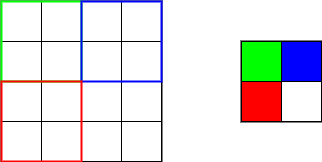
\includegraphics[scale=0.5]{stride.png}
    \caption{Primjer konvolucije s korakom 2}
    \label{fig:stride}
\end{figure}

Na slici~\ref{fig:stride} moguće je vidjeti konvoluciju s korakom 2. Za razliku od standardnog kretanja jezgre, ovdje se jezgra nakon svakog izračuna pomiče za 2 ćelije. 

Osim samih konvolucijskih slojeva, konvolucijske mreže u sebi sadrže i slojeve sažimanja. 
Najčešći razlog za upotrebu slojeva sažimanja je smanjivanje dimenzija podataka, a time i skraćivanje vremena potrebnog za učenje mreže.

\begin{figure}[htb]
    \centering
    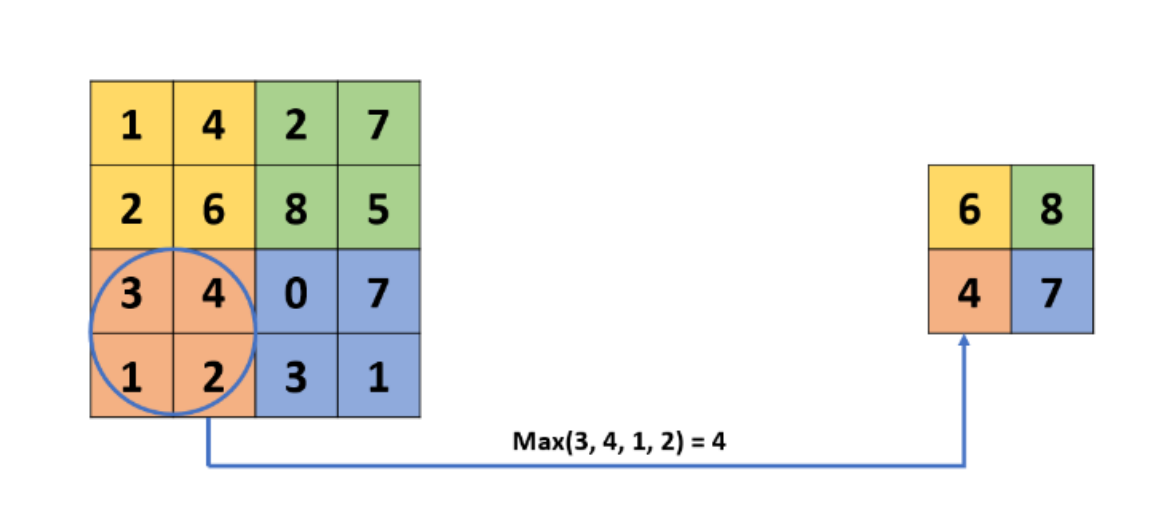
\includegraphics[scale=0.35]{maxpool.png}
    \caption{Primjer sažimanja maksimalnom vrijednošću. Preuzeto iz \cite{gholamalinezhad2020pooling}}
    \label{fig:maxpool}
\end{figure}

Na slici~\ref{fig:maxpool} moguće je vidjeti primjer korištenja sloja sažimanja maksimalnom vrijednošću.
Mapa značajki dimenzija 4x4 korištenjem sažimanja maksimalnom vrijednošću 2x2 (engl.\ \textit{2x2 max pooling}) smanjena je na dimenzije 2x2, efektivno smanjujući dimenzije ulaza za faktor 2.
Uz sažimanje maksimalnom vrijednošću, veoma je popularno i sažimanje usrednjavanjem, no postoje i brojne druge varijante koje se koriste za slojeve sažimanja.
Kao i operacija konvolucije, i slojevi sažimanja doprinose translacijskoj invarijantnosti, osiguravajući da mreža lako može prepoznati neku značajku bez obzira na njenu točnu lokaciju.

\section{Rezidualne mreže}

Rezidualne mreže~\cite{he2016deep} vrsta su dubokih neuronskih mreža koje koriste rezidualne blokove. Općenito govoreći, blok u kontekstu neuronskih mreža označava niz od nekoliko slojeva. 
Pojedini blokovi mogu se kombinirati kako bi sačinjavali složeniju mrežu. 
Rezidualni blokovi najčešće se sastoje od nekoliko konvolucijskih slojeva, a njihova glavna karakteristika postojanje je preskočnih veza.

\begin{figure}[htb]
    \centering
    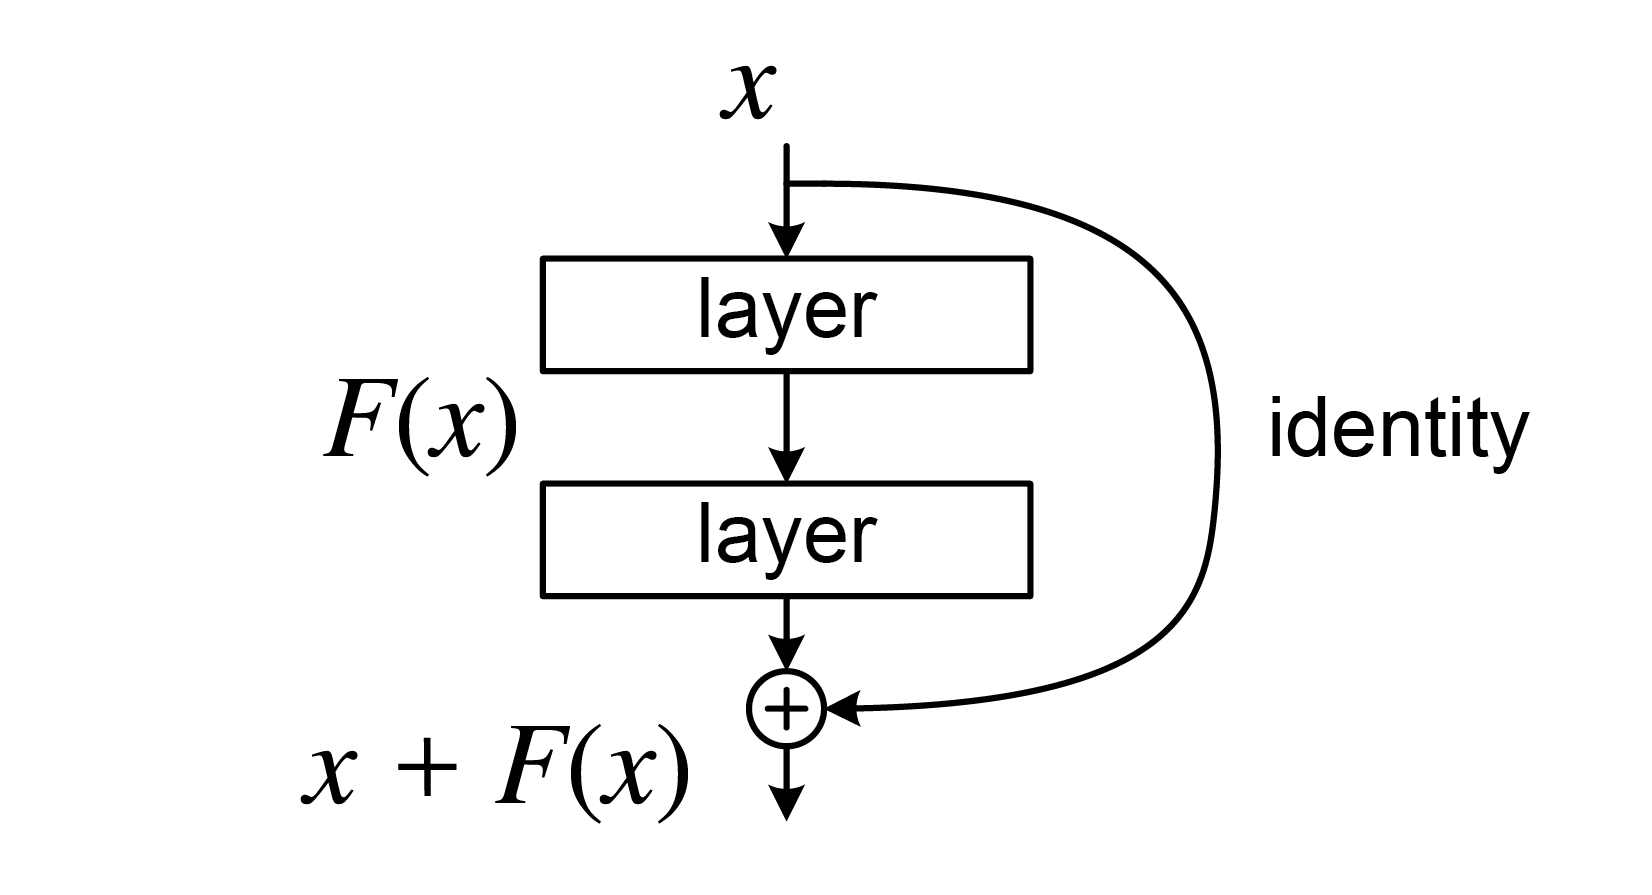
\includegraphics{ResBlock.png}
    \caption{Primjer rezidualnog bloka. Preuzeto iz \cite{he2016deep}}
    \label{fig:resblock}
\end{figure}

Na slici~\ref{fig:resblock} možemo vidjeti rezidualni blok sačinjen od dva sloja. Preskočna veza ulaz u blok bez ikakvih transformacija prenosi na izlaz. 
Ovakvim strukturiranjem mreže, cilj mreže postaje modelirati rezidualnu funkciju $F(x)$ koja mjeri razliku izlaza naspram ulaza. Rezidualni blok možemo prikazati jednadžbom:

\begin{equation}
    f(\pmb{x}) = F(\pmb{x}) + \pmb{x}
    \label{eq:resblock}
\end{equation}
\\
pri čemu $F(x)$ predstavlja rezidualnu funkciju, $x$ prenošenje ulaza na izlaz preskočnom vezom, a $f(x)$ izlaz bloka. 
U slučaju da slojevi između mijenjaju dimenzije podataka, preskočna veza morat će raditi linearnu projekciju kako bi podatci pri zbrajanju bili istih dimenzija. 
Tada rezidualni blok možemo prikazati na sljedeći način:

\begin{equation}
    f(\pmb{x}) = F(\pmb{x}) + \pmb{W}_{s} \cdot \pmb{x}
    \label{eq:resblocklp}
\end{equation}
\\
pri čemu $W_{s}$ označava matricu korištenu za linearnu projekciju ulaza $x$. 
Korištenje slojeva s preskočnim vezama motivirano je željom za učenjem funkcije identiteta.
Klasične duboke mreže s velikim brojem slojeva teško će naučiti funkciju identiteta, dok korištenje preskočnih veza dubokim mrežama značajno olakšava učenje te funkcije.
Ovo potječe od činjenice da je za uspješno modeliranje funkcije identiteta $f(x)$ za rezidualnu funkciju $F(x)$ potrebno samo postaviti težine jezgri na 0.

\section{ResNet18}

U okviru ovog rada, za provođenje svih eksperimenata koristit ćemo ResNet18 mrežu kako bismo što bolje mogli usporediti učinak različitih eksperimenata. 
ResNet18 rezidualna je neuronska mreža, a sastoji se od ukupno 18 slojeva. 

\begin{figure}[htb]
    \centering
    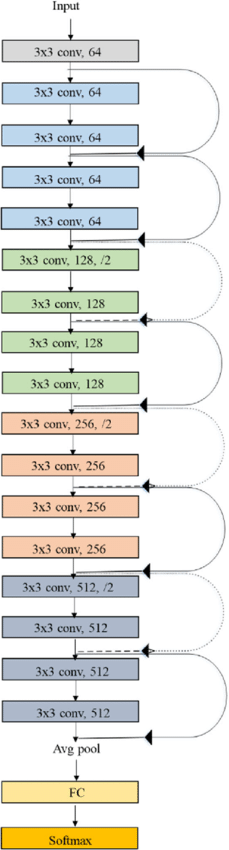
\includegraphics[scale=0.7]{resnet18.png}
    \caption{Arhitektura ResNet18. Preuzeto iz \cite{mcc19}}
    \label{fig:resnet18}
\end{figure}

Kao što možemo vidjeti na slici~\ref{fig:resnet18}, ResNet18 sastoji se od 8 rezidualnih blokova. Svaki od tih blokova sastoji se od 2 konvolucijska sloja i jedne preskočne veze.
Rezidualnim blokovima prethodi jedan konvolucijski sloj, a nakon njih dolazi jedan potpuno-povezani sloj sa softmax prijenosnom (aktivacijskom) funkcijom.

\chapter{Brzo učenje s neprijateljskim primjerima}

\section{Neprijateljski primjeri}

Kada učimo modele da rješavaju razne probleme, cilj nam je da modeli pokažu svojstvo generalizacije. 
U slučaju problema klasifikacije, to znači da bi modeli trebali dobro klasificirati i do sada neviđene primjere.
Mogućnost generalizacije određenog modela najčešće provjeravamo koristeći unakrsnu provjeru (engl.\ \textit{cross-validation}).
Pritom skup podataka dijelimo na 2 ili 3 skupa: 

\begin{enumerate}
    \item skup za učenje (engl.\ \textit{train set})
    \item skup za provjeru (engl.\ \textit{validation set})
    \item skup za testiranje (engl.\ \textit{test set})
\end{enumerate}

Skup za učenje modelu predočavamo kako bi na temelju njega mogao poboljšavati svoje parametre tj.\ učiti. 
S druge strane, skup za provjeru koristimo za poboljšavanje hiperparametara modela (npr.\ stopa učenja modela). 
U slučaju da smo sigurni u dobar odabir hiperparametara modela, korištenje ovog skupa nije nužno. 
Nakon postupka učenja, koristeći skup za testiranje evaluiramo model.

Općenito govoreći, model će na skupu za testiranje postizati lošije rezultate naspram rezultata na skupu za učenje. 
Ako model dobro generalizira, razlika između rezultata na ta dva skupa neće biti veoma značajna. 
Ipak, u zadnjih desetak godina otkriveni su ulazi koje i modeli koji inače pokazuju mogućnost generalizacije loše klasificiraju.
Takve ulaze zvat ćemo neprijateljski primjeri~\cite{goodfellow2014explaining}.

\pagebreak

\begin{figure}[htb]
    \centering
    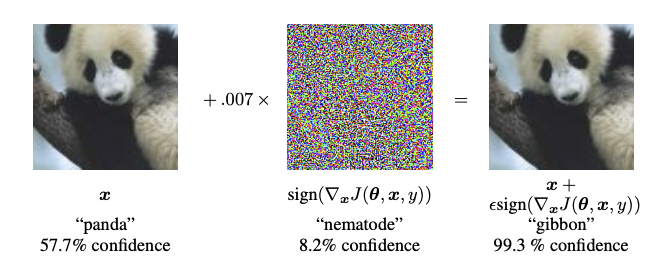
\includegraphics[scale=0.5]{adversarial_example.png}
    \caption{Primjer neprijateljskog primjera. Preuzeto iz \cite{goodfellow2014explaining}}
    \label{fig:adv_example}
\end{figure}

Na slici~\ref{fig:adv_example} moguće je vidjeti jedan neprijateljski primjer.
Originalni ulaz kojeg model ispravno klasificira izmijenjen je za iznos perturbacije.
U ovom slučaju iznos perturbacije dobiven je kao umnožak malog pozitivnog koeficijenta $\epsilon$ i predznaka gradijenta gubitka po ulazu.
Iako je izmijenjeni ulaz ljudima gotovo identičan, model ovaj ulaz krivo klasificira, a pritom je veoma siguran u svoju odluku.
Ovo svojstvo iskazali su brojni modeli te je zbog toga u zadnjih desetak godina porastao interes za proučavanjem neprijateljskih primjera.

\section{Načini generiranja neprijateljskih primjera}

Neprijateljske primjere moguće je generirati na različite načine. 
Načine generiranja neprijateljskih primjera zovemo napadima, a možemo ih podijeliti na usmjerene i neusmjerene napade.
Usmjereni napadi kao cilj imaju generiranje neprijateljskih primjera koje će napadnuti model klasificirati u točno jedan ciljni razred,
dok neusmjereni napadi kao cilj imaju generiranje neprijateljskih primjera koje će napadnuti model što lošije klasificirati, neovisno o konkretnom razredu.
Pronalaženje neprijateljskih primjera zapravo je optimizacijski problem koji možemo prikazati sljedećim izrazom:

\begin{equation}
    \underset{\delta \in [-\epsilon, \epsilon]}{max}L(x + \delta,y;\theta)
    \label{eq:adversarial_optimization}
\end{equation}
\\
pri čemu $\delta$ označava iznos perturbacije u intervalu određenim s granicama $[-\epsilon, \epsilon]$, $L(x,y;\theta)$ funkciju gubitka, a $\theta$ parametre modela.
Drugim riječima, cilj nam je naći perturbaciju omeđenu određenim iznosom takvu da je iznos funkcije gubitka za ulaz izmijenjen tom perturbacijom maksimalan.
Iznos perturbacije najčešće je omeđen L\textsubscript{$\infty$}-normom, no isti može biti omeđen i L\textsubscript{2}-normom ili L\textsubscript{1}-normom.

Postoje brojni načini generiranja neprijateljskih primjera. 
Neki od najpoznatijih su FGSM (engl.\ \textit{Fast Gradient Sign Method})~\cite{goodfellow2014explaining} i PGD (engl.\ \textit{Projected Gradient Descent})~\cite{madry2017towards} napadi.
Primjer sa slike~\ref{fig:adv_example} zapravo je neprijateljski primjer generiran koristeći FGSM napad, a neprijateljske primjere generirane koristeći taj napad sažeto možemo opisati jednadžbom:

\begin{equation}
    x := x + \epsilon \cdot sign(\nabla_{x}L(x,y;\theta))
    \label{eq:fgsm}
\end{equation}
\\
pri čemu $\epsilon$ predstavlja mali pozitivan broj koji određuje veličinu perturbacije, a $sign(x)$ predznak od $x$. 
FGSM napad originalnom ulazu pridodaje iznos istog predznaka kao i gradijent funkcije gubitka, time osiguravajući najveći mogući rast iznosa funkcije gubitka. 
U slučaju neusmjerenog napada, napad bi pokušavao što više smanjiti iznos funkcije gubitka s obzirom na proizvoljan razred.

Uz FGSM napad, postoji i napad koji iterativno stvara značajno učinkovitije neprijateljske primjere. 
Tu vrstu napada zovemo PGD napad, a zasniva se na istoj ideji kao i FGSM napad. 
Za razliku od FGSM-a, PGD napad iterativno ponavlja postupak, time pokušavajući odrediti najbolje rješenje optimizacijskog problema~\ref{eq:adversarial_optimization}.
Uz to, PGD napad tijekom generiranja neprijateljskih primjera osigurava da ukupna perturbacija nije veća od unaprijed definiranog koeficijenta $\epsilon$.

\begin{algorithm}
    \caption{Generiranje neprijateljskih primjera koristeći PGD napad}
    \label{algo:pgd}
    \begin{algorithmic}
        \STATE{\textbf{Ulaz:} $x$ -- ulazne slike, $y$ -- ispravne oznake ulaznih slika, $\epsilon$ -- ograničenje perturbacije, $\alpha$ -- veličina koraka po iteraciji, $K$ -- broj iteracija za generiranje neprijateljskih primjera}
        \STATE{\textbf{Izlaz:} $x_{adv}$ -- neprijateljski primjeri generirani PGD napadom}
        \\\hrulefill
        \STATE{$\delta = U(-\epsilon, \epsilon)$}
        \FOR{($i = 1 \dots K$)}
            \STATE{$grad = \nabla_{\delta}L(x + \delta,y;\theta)$}
            \STATE{$\delta = \delta + \alpha \cdot sign(g)$}
            \STATE{$\delta = clamp(\delta, -\epsilon, \epsilon)$}
        \ENDFOR
        \STATE{$x_{adv} = x + \delta$}
        \RETURN{$x_{adv}$}
    \end{algorithmic}
\end{algorithm}

\pagebreak

Pseudokod~\ref{algo:pgd} prikazuje način generiranja neprijateljskih primjera koristeći PGD napad. 
Perturbacija $\delta$ na početku je inicijalizirana koristeći uniformnu distribuciju s rasponom $[-\epsilon, \epsilon]$, 
a na kraju svake iteracije iznos perturbacije ograničava se koristeći funkciju \textit{clamp}. 
Naravno, postoje brojni načini inicijalizacije iznosa perturbacije, no nasumična inicijalizacija pokazala se dosta uspješnom.
Važno je istaknuti da pseudokod za ograničavanje iznosa perturbacije koristi L\textsubscript{$\infty$}-normu. 
PGD napad s $K$ iteracija za generiranje neprijateljskih primjera zvat ćemo K-PGD (npr.\ 20-PGD).

\section{Učenje s neprijateljskim primjerima}

Ako želimo da modeli koje učimo budu otporni na neprijateljske primjere tj.\ ispravno ih klasificiraju, ne možemo se ograničiti na klasično (prirodno) učenje modela.
Svojstvo otpornosti na neprijateljske primjere zvat ćemo robusnost, a jedan od mogućih načina za postizanje robusnih modela učenje je s neprijateljskim primjerima (robusno učenje).
Kada govorimo o učenju s neprijateljskim primjerima, općenita ideja je da se tijekom učenja generiraju neprijateljski primjeri prilagođeni samome modelu.
Model tada ne uči na originalnim ulaznim podacima, već isključivo na generiranim neprijateljskim primjerima.
U tom slučaju neprijateljske primjere možemo smatrati načinom augmentacije ulaznih podataka - na temelju originalnih ulaznih podataka stvaramo nove podatke koje predočavamo modelu.

Robusnim učenjem možemo postići puno višu točnost modela na skupu za testiranje sačinjenom od neprijateljskih primjera naspram modela učenih prirodnim učenjem.
Nažalost, robusno učenje ima svoju cijenu. Robusni modeli gotovo uvijek će na originalnom skupu za testiranje imati nižu točnost naspram modela učenih prirodnim učenjem,
a i učit će se dulje. Ako za generiranje neprijateljskih primjera tijekom robusnog učenja koristimo FGSM metodu, učenje će trajati otprilike dvostruko dulje naspram prirodnog učenja
jer je za generiranje neprijateljskih primjera FGSM metodom potreban dodatan unaprijedni prolaz kroz mrežu. 
Ako za generiranje neprijateljskih primjera koristimo PGD metodu, duljina trajanja učenja ovisit će o broju iteracija korištenih za generiranje neprijateljskih primjera.
Koristimo li 10 iteracija za generiranje neprijateljskih primjera, učenje će trajati otprilike 11 puta dulje naspram prirodnog učenja. 
Općenito govoreći, kako bismo model učili koristeći neprijateljske primjere generirane K-PGD metodom, učenje će trajati otprilike K + 1 puta dulje naspram prirodnog učenja~\cite{shafahi2019adversarial}.

\pagebreak

\begin{algorithm}
    \caption{Učenje s neprijateljskim primjerima}
    \label{algo:adv_learning}
    \begin{algorithmic}
        \STATE{\textbf{Ulaz:} $x$ -- ulazne slike, $y$ -- ispravne oznake ulaznih slika, $N$ -- broj epoha, $M$ -- veličina skupa za učenje, $K$ -- broj iteracija za generiranje neprijateljskih primjera, $\eta$ -- stopa učenja, $\epsilon$ -- ograničenje perturbacije, $\alpha$ -- veličina koraka po iteraciji}
        \\\hrulefill
        \STATE{$\theta = initializeModelParams()$}
        \FOR{$(ep = 1 \dots N)$}
            \FOR{$(i = 1 \dots M)$}
                \STATE{$x_{adv} = generateAdversarial(x_{i}, y_{i}, \epsilon, \alpha, K)$}
                \STATE{$grad = \nabla_{\theta}L(x_{adv},y_{i};\theta)$}
                \STATE{$\theta = \theta - \eta \cdot grad$}
            \ENDFOR
        \ENDFOR
    \end{algorithmic}
\end{algorithm}

Pseudokod~\ref{algo:adv_learning} prikazuje općeniti algoritam za učenje s neprijateljskim primjerima.
Pritom inicijalizaciju parametara modela $\theta$ prikazujemo pozivom funkcije \textit{initializeModelParams}.
Radi općenitosti, generiranje neprijateljskih primjera prikazano je pozivom funkcije \textit{generateAdversarial}.
Ta funkcija mogla bi generirati neprijateljske primjere koristeći FGSM metodu, PGD metodu ili neki alternativan način, no to nam za općeniti prikaz nije važno.

\section{Brzo učenje s neprijateljskim primjerima}

U slučaju da model koji učimo nije veoma složen, obično učenje s neprijateljskim primjerima prihvatljiv je način za postizanje robusnih modela otpornih na napade.
Ipak, ako učimo složene modele na velikim skupovima podataka, obično učenje s neprijateljskim primjerima presporo je. 
Uz to, rijetko tko uopće posjeduje dovoljnu količinu računalnih resursa za robusno učenje složenijih modela.
Kako bismo riješili ili barem umanjili ovaj problem, predložena su brojna rješenja čijom bi se primjenom ubrzalo robusno učenje. Razmotrit ćemo tri takva rješenja.

\pagebreak

\subsection{Besplatno učenje}

Jedno od prvih predloženih rješenja za problem duljine trajanja učenja robusnih modela naziva se besplatno učenje (engl.\ \textit{free adversarial training})~\cite{shafahi2019adversarial}.
Uočeno je da modeli učeni koristeći neprijateljske primjere generirane PGD metodom imaju visoku robusnost, no, kao što je već rečeno, zahtijevaju puno vremena za učenje.

Osnovna ideja besplatnog učenja je sljedeća: unatražnim prolazom osim iznosa gradijenta po parametrima modela izračunamo i iznos gradijenta po ulazu potreban za generiranje neprijateljskih primjera.
Kako bi se neprijateljski primjeri iterativno izmjenjivali, na svakoj mini-grupi model uči nekoliko puta zaredom. Ovaj hiperparametar zovemo ponavljanje (engl.\ \textit{replay}).
Važno je uočiti da, kako bismo i dalje trebali otprilike jednako vremena za učenje modela, moramo smanjiti broj epoha za faktor ponavljanja. 
Ako svaku mini-grupu unutar jedne epohe ponavljamo 8 puta, broj epoha bit će 8 puta manji naspram broja epoha kod modela učenog prirodnim učenjem.
Nažalost, povećavanjem broja ponavljanja dolazi do degradacije performansi modela na običnom testnom skupu - u pitanju je kompromis između željene razine robusnosti i točnosti na običnom testnom skupu.

\begin{algorithm}
    \caption{Besplatno učenje s neprijateljskim primjerima. Prilagođeno iz~\cite{wong2020fast}}
    \label{algo:adv_learning_free}
    \begin{algorithmic}
        \STATE{\textbf{Ulaz:} $x$ -- ulazne slike, $y$ -- ispravne oznake ulaznih slika, $N$ -- broj epoha, $M$ -- veličina skupa za učenje,  $K$ -- broj ponavljanja (engl.\ \textit{replay}), $\eta$ -- stopa učenja, $\epsilon$ -- ograničenje perturbacije}
        \\\hrulefill
        \STATE{$\theta = initializeModelParams()$}
        \STATE{$\delta = 0$}
        \FOR{$(ep = 1 \dots N/K)$}
            \FOR{$(i = 1 \dots M)$}
                \FOR{$(j = 1 \dots K)$}
                    \STATE{$gradAdv, grad = \nabla L(x_{i} + \delta,y_{i};\theta)$}
                    \STATE{$\delta = \delta + \epsilon \cdot sign(gradAdv)$}
                    \STATE{$\delta = clamp(\delta, -\epsilon, \epsilon)$}
                    \STATE{$\theta = \theta - \eta \cdot grad$}
                \ENDFOR
            \ENDFOR
        \ENDFOR
    \end{algorithmic}
\end{algorithm}

\pagebreak

Pseudokod~\ref{algo:adv_learning_free} prikazuje algoritam za besplatno učenje s neprijateljskim primjerima.
Kao i u prethodnom algoritmu, parametri modela $\theta$ inicijaliziraju se pozivom funkcije \textit{initializeModelParams}.
Važno je uočiti da se iznosi gradijenata potrebni za generiranje neprijateljskih primjera, ali i izmjenu parametara modela izračunavaju u istom unatražnom prolazu,
time osiguravajući da generiranje neprijateljskih primjera ne usporava postupak učenja. 
Uz to, perturbacija $\delta$ inicijalizira se na 0 samo na početku postupka učenja - kada započinje izračun perturbacije za sljedeći ulaz, prethodni iznos služi kao "iznos za zagrijavanje" (engl.\ \textit{warmup}).

Ovakvim načinom robusnog učenja, duljina trajanja učenja modela otprilike je jednaka kao i duljina trajanja učenja modela prirodnim učenjem.
Uz to, rezultati rada~\cite{shafahi2019adversarial} pokazuju da je robusnost naučenih modela usporediva s robusnošću modela učenih koristeći neprijateljske primjere generirane PGD metodom.
Kao što je već rečeno, visoku robusnost modela učenih koristeći besplatno učenje možemo postići izmjenom broja ponavljanja, ali po cijeni smanjenja performansi modela na običnom testnom skupu.

\subsection{Brzo učenje}

Za modele učene koristeći FGSM metodu dugo se smatralo da nisu otporni na neprijateljske primjere generirane koristeći iterativne metode poput PGD-a.
Takvi modeli nisu nam veomi korisni jer često imaju nižu točnost na običnim podatcima, a ne nude pravu mjeru robusnosti - napadač jednostavno može generirati neprijateljske primjere koje će model krivo klasificirati.
Ipak, rad~\cite{wong2020fast} predlaže da problem ne leži u korištenju FGSM metode, već njenoj inicijalizaciji.
Standardno se perturbacija za FGSM metodu inicijalizira na 0 ili na granicu perturbacije $\epsilon$, bilo s pozitivnim ili negativnim predznakom.
U slučaju da za inicijalizaciju iskoristimo nasumičnu inicijalizaciju koristeći uniformnu distribuciju s granicama $[-\epsilon, \epsilon]$, 
modeli učeni koristeći FGSM metodu postižu svojstvo robusnosti čak i protiv iterativnih napada.

Ako učenje koristeći FGSM metodu s nasumičnom inicijalizacijom kombiniramo s nekim od mogućih optimizacija poput korištenja cikličke stope učenja i računanja u mješovitoj preciznosti,
dobivamo tzv.\ brzo učenje (engl.\ \textit{fast adversairal training})~\cite{wong2020fast}. Predložene optimizacije omogućavaju značajno ubrzanje učenja modela, a nisu implementacijski zahtjevne.
Ciklička stopa učenja~\cite{smith2017cyclical} označava promjenu stope učenja kroz epohe ili iteracije - nakon svakog koraka, stopa učenja će se povećavati ili smanjivati unutar unaprijed definiranih granica.
Uvođenje cikličke stope učenja korisno je za brže konvergiranja modela, time ubrzavajući učenje. 
Uz cikličku, postoje i brojne druge poput linearne i kosinusne, no brzo učenje koristi upravo cikličku stopu učenja.

Razvoj tenzorskih jezgri grafičkih kartica omogućilo je korištenje računanja u mješovitoj preciznosti - 
umjesto da se svi izračuni obavljaju koristeći 32-bitne brojeve s pomičnim zarezom, neki izračuni obavljaju se koristeći 16-bitne brojeve.
Korištenjem računanja u mješovitoj preciznosti, značajno se može ubrzati učenje, ali i smanjiti potrebna količina memorije za učenje modela.
Naravno, da bismo isto mogli koristiti, grafičke kartice na kojim učimo modele moraju imati tenzorske jezgre. Ako koristimo starije grafičke kartice, učenje neće biti brže.

\begin{algorithm}
    \caption{Brzo učenje s neprijateljskim primjerima. Prilagođeno iz~\cite{wong2020fast}}
    \label{algo:adv_learning_fast}
    \begin{algorithmic}
        \STATE{\textbf{Ulaz:} $x$ -- ulazne slike, $y$ -- ispravne oznake ulaznih slika, $N$ -- broj epoha, $M$ -- veličina skupa za učenje, $\eta$ -- stopa učenja, $\epsilon$ -- ograničenje perturbacije, $\alpha$ -- veličina koraka}
        \\\hrulefill
        \STATE{$\theta = initializeModelParams()$}
        \FOR{$(ep = 1 \dots N)$}
            \FOR{$(i = 1 \dots M)$}
                \STATE{$\delta = U(-\epsilon, \epsilon)$}
                \STATE{$gradAdv = \nabla_{\delta}L(x_{i} + \delta,y_{i};\theta)$}
                \STATE{$\delta = \delta + \alpha \cdot sign(gradAdv)$}
                \STATE{$\delta = clamp(\delta, -\epsilon, \epsilon)$}
                \STATE{$grad = \nabla_{\theta}L(x_{i} + \delta,y_{i};\theta)$}
                \STATE{$\theta = \theta - \eta \cdot grad$}
            \ENDFOR
        \ENDFOR
    \end{algorithmic}
\end{algorithm}

Pseudokod~\ref{algo:adv_learning_fast} prikazuje algoritam za brzo učenje s neprijateljskim primjerima.
Kao i prije, parametri modela $\theta$ inicijaliziraju se pozivom funkcije \textit{initializeModelParams}.
Početni iznos perturbacije $\delta$ inicijalizira se koristeći uniformnu distribuciju s rasponom $[-\epsilon, \epsilon]$.
Za razliku od besplatnog učenja, kod brzog učenja potrebna su dva unaprijedna prolaza, kao i dva zasebna izračuna iznosa gradijenta za svaki ulaz.
Zbog ovoga brzo učenje nije jednako brzo kao i prirodno učenje modela, ali zato nudi određenu mjeru robusnosti.

Prema radu~\cite{wong2020fast}, brzo učenje modela nudi gotovo jednaku mjeru robusnosti protiv iterativnih napada kao i modeli učeni koristeći PGD metodu, 
ali sa značajno kraćim vremenom učenja. Čak i ako već navedene optimizacije primijenimo na besplatno učenje i učenje koristeći PGD metodu, 
da bismo postigli jednaku mjeru robusnosti modele je potrebno učiti dulje nego modele učene koristeći brzo učenje.

Nažalost, korištenje brzog učenja s neprijateljskim primjerima ima i svoju manu. U slučaju da modele učimo velik broj epoha,
u jednom trenutku gotovo sigurno će doći do značajnog pada u točnosti na neprijateljskim primjerima. Ovu pojavu zovemo katastrofalna prenaučenost (engl.\ \textit{catastrophic overfitting}),
a jedan od mogućih načina za sprječavanje iste je korištenje ranog završetka (engl.\ \textit{early stopping}). 
Kako bismo na vrijeme mogli zaustaviti učenje modela, nakon svake epohe evaluiramo točnost modela na neprijateljskim primjerima generiranim iz nasumične mini-grupe.
U slučaju da je točnost u trenutnoj epohi značajno manja od točnosti u prethodnoj epohi, zaustavljamo učenje modela i kao najbolji model vraćamo model iz prethodne epohe.
Zbog ovog svojstva, korištenje brzog učenja s neprijateljskim primjerima nije prikladno za modele koje trebamo učiti velik broj epoha.

\subsection{Nadogradnje brzog učenja}

Kako bi brzo učenje s neprijateljskim primjerima bilo primjenjivo za proizvoljno dugo učenje, potrebno je riješiti problem katastrofalne prenaučenosti.
Taj problem pojavljuje se kod svih postupaka koji koriste FGSM metodu za učenje, no manje je izražen kod brzog učenja nego kod običnog učenja s neprijateljskim primjerima generiranim koristeći FGSM metodu.
Rad~\cite{li2020towards} otkriva nam da brzo učenje u manjoj mjeri pati od problema katastrofalne prenaučenosti zbog nasumične inicijalizacije perturbacije.
Kao i kod modela učenih običnim FGSM-om, i modeli učeni koristeći brzo učenje susreću se s katastrofalnom prenaučenošću, ali se od iste u periodu od nekoliko mini-grupa mogu oporaviti te nastaviti dalje normalno učiti.

Ključ u oporavku leži u nasumičnoj inicijalizaciji koja pomaže u stvaranju kvalitetnih neprijateljskih primjera. 
Ipak, zbog nasumičnosti nemamo garanciju da će takav postupak uvijek biti dovoljan za oporavak pa nakon određene količine vremena i dalje dođe do katastrofalne prenaučenosti.
Ako bismo mogli garantirati da će se model tijekom učenja uvijek moći oporaviti od katastrofalne prenaučenosti u periodu od nekoliko mini-grupa, mogli bismo proizvoljno dugo učiti model.
U radu~\cite{li2020towards} oporavak se postiže kontinuiranim praćenjem točnosti na neprijateljskim primjerima generiranim iz nasumične mini-grupe svakih $s$ mini-grupa. 
U slučaju da je točnost u trenutnom koraku značajno manja od točnosti u prethodnom koraku, do sljedeće provjere točnosti umjesto FGSM metode s nasumičnom inicijalizacijom, za generiranje neprijateljskih primjera koristimo PGD metodu.
Ovakvim postupkom model se lako može oporaviti od pojave katastrofalne prenaučenosti pa stoga može i dulje učiti.



\chapter{Zaključak}
Zaključak.

\bibliography{literatura}
\bibliographystyle{fer}

\begin{sazetak}
Sažetak na hrvatskom jeziku.

\kljucnerijeci{Ključne riječi, odvojene zarezima.}
\end{sazetak}

% TODO: Navedite naslov na engleskom jeziku.
\engtitle{Algorithms for fast robust training on adversarial examples}
\begin{abstract}
Abstract.

\keywords{Keywords.}
\end{abstract}

\end{document}
